% -*- latex -*-
%%%%%%%%%%%%%%%%%%%%%%%%%%%%%%%%%%%%%%%%%%%%%%%%%%%%%%%%%%%%%%%%
%%%%%%%%%%%%%%%%%%%%%%%%%%%%%%%%%%%%%%%%%%%%%%%%%%%%%%%%%%%%%%%%
%%%%
%%%% This text file is part of the source of 
%%%% `Parallel Computing'
%%%% by Victor Eijkhout, copyright 2012-6
%%%%
%%%% mpi-data.tex : discussion of MPI datatypes
%%%%
%%%%%%%%%%%%%%%%%%%%%%%%%%%%%%%%%%%%%%%%%%%%%%%%%%%%%%%%%%%%%%%%
%%%%%%%%%%%%%%%%%%%%%%%%%%%%%%%%%%%%%%%%%%%%%%%%%%%%%%%%%%%%%%%%

\Level 0 {MPI Datatypes}

\index{datatype|(}

In the examples you have seen so far, every time data was sent,
it was as a contiguous buffer with elements of a single type.
In practice you may want to send heterogeneous data, or
non-contiguous data.
Figure~\ref{fig:blasmatrix} indicates one source of irregular
data:
%
\begin{figure}[ht]
  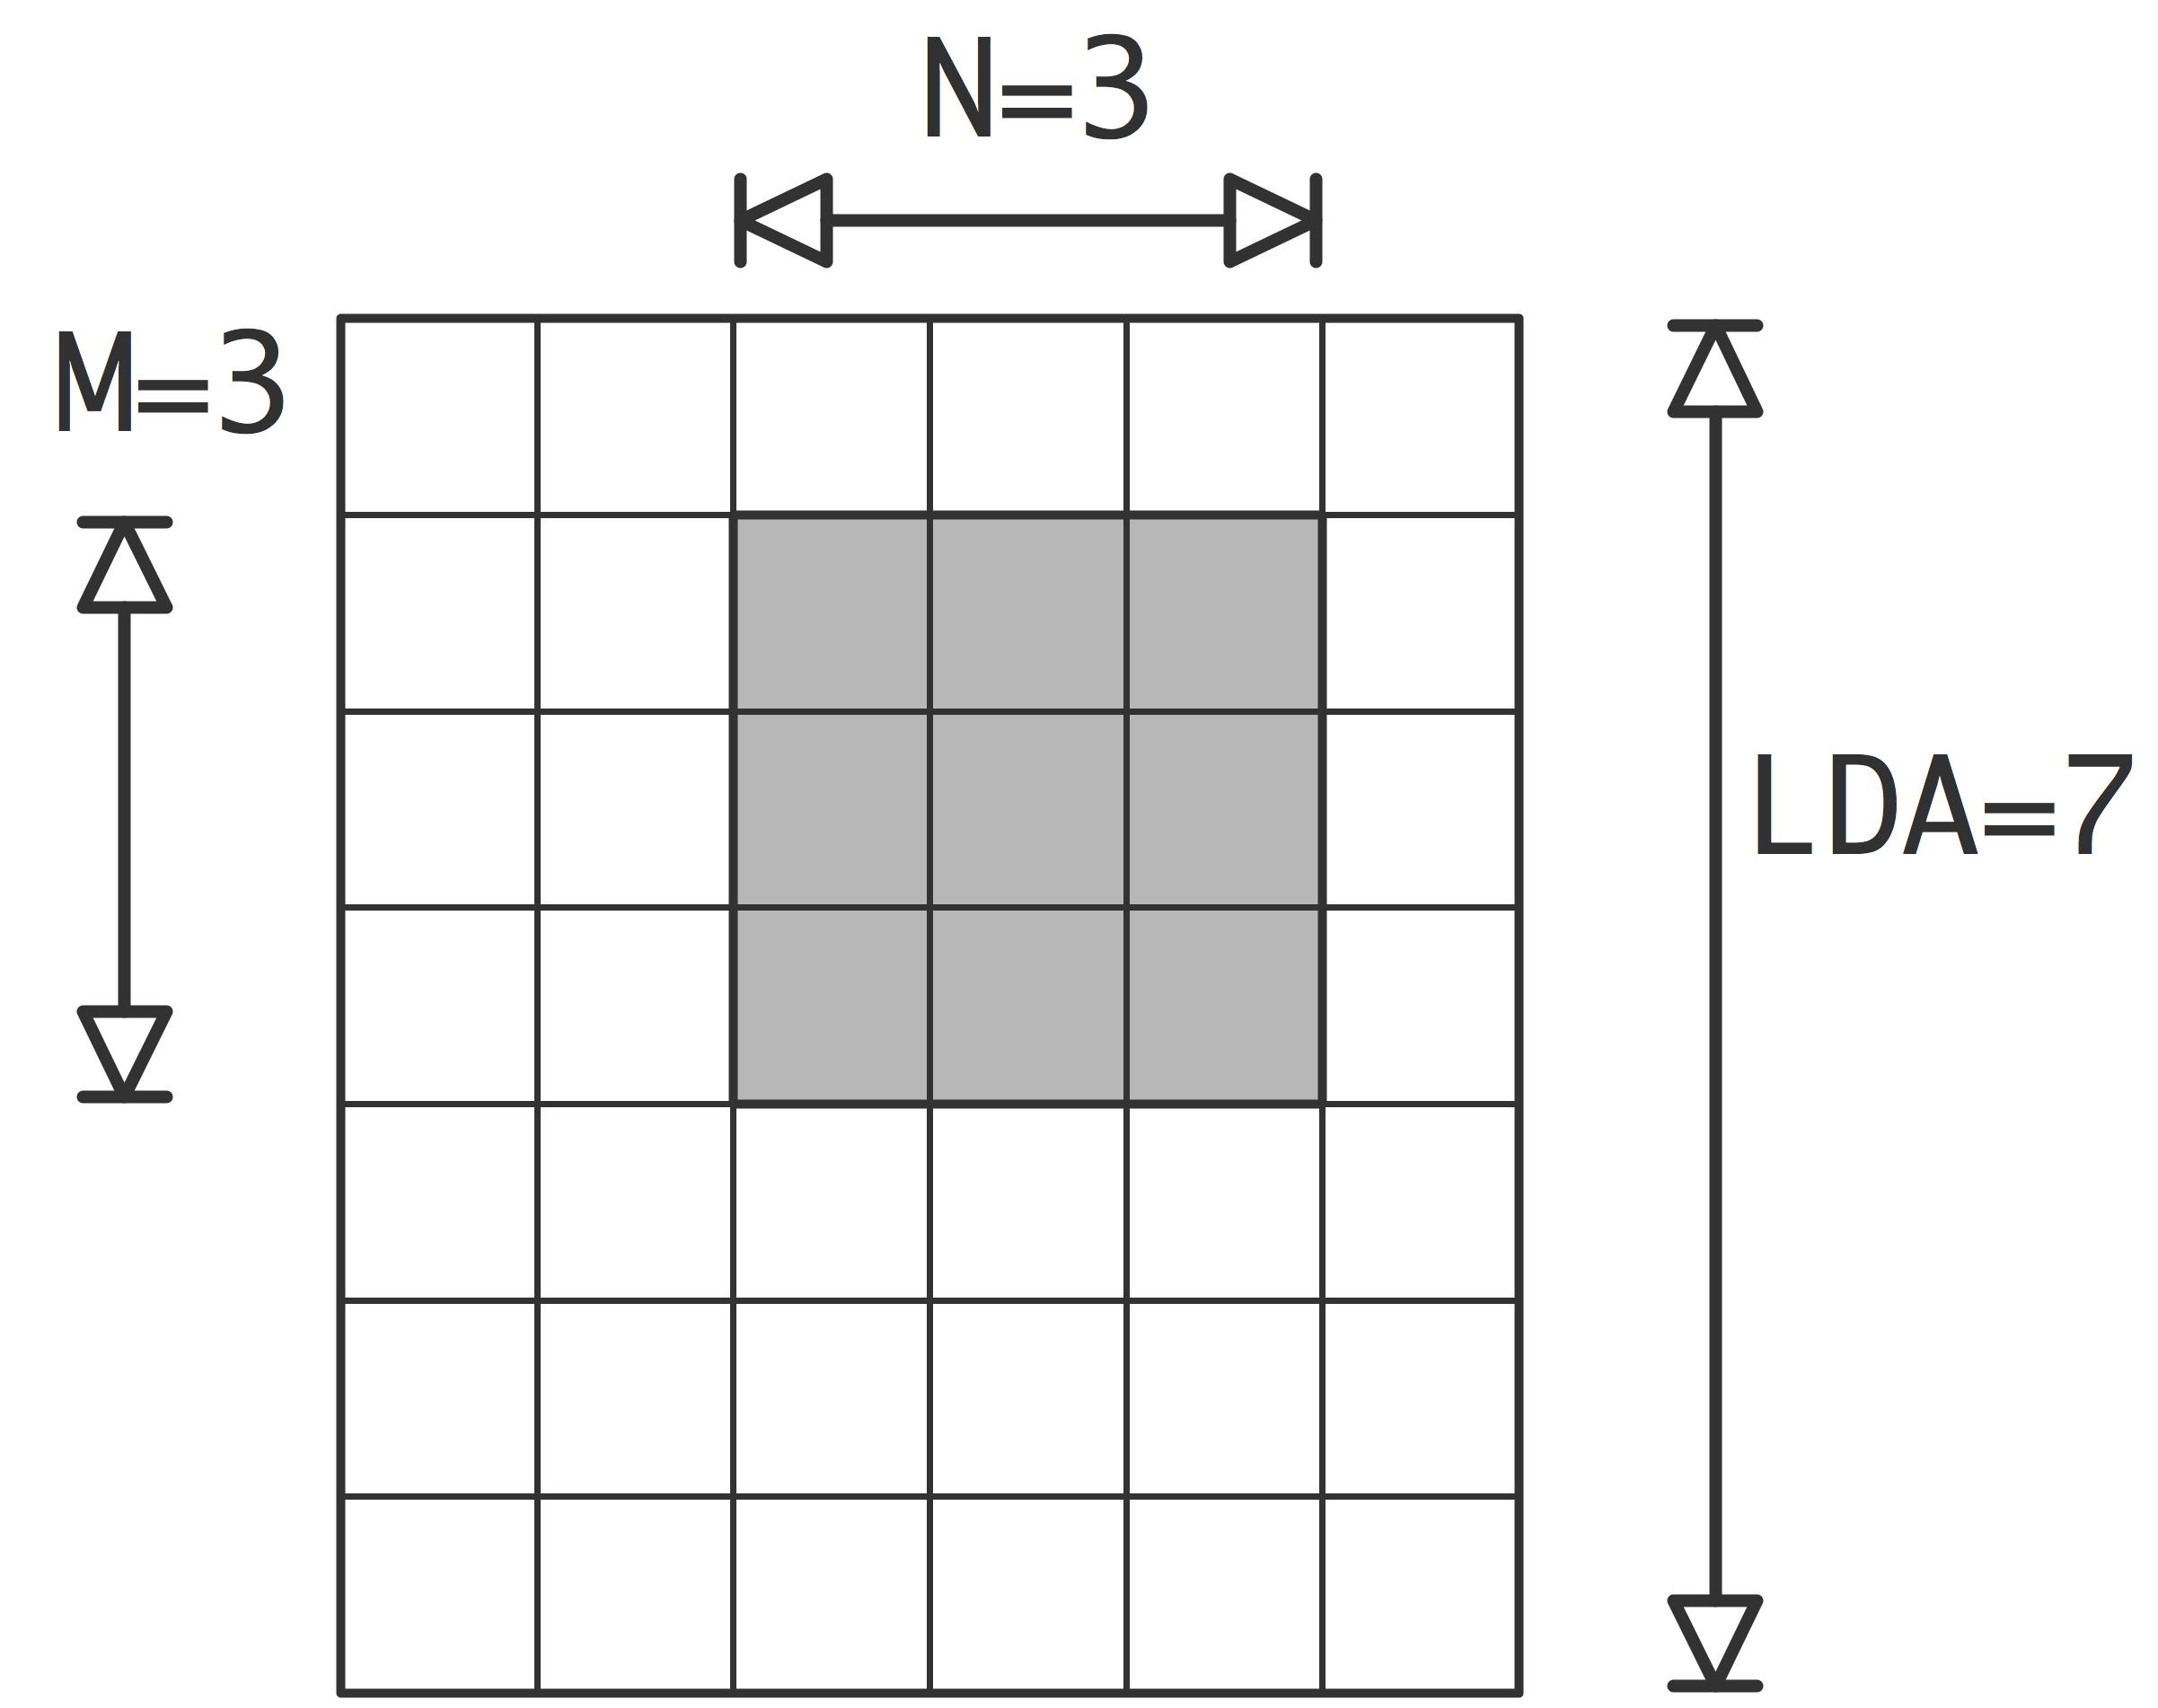
\includegraphics[scale=.1]{blasmatrix}
  \caption{Memory layout of a row and column of a matrix in column-major storage}
  \label{fig:blasmatrix}
\end{figure}
%
with a matrix on \indexterm{column-major storage}, a column is
stored in contiguous memory. However, a row of such a matrix
is not contiguous; its elements being separated by a \indexterm{stride}
equal to the column length.

\begin{exercise}
  \label{ex:submatrix}
  How would you describe the memory layout of a submatrix,
  if the whole matrix has size $M\times N$ and the submatrix $m\times n$?
\end{exercise}

The datatypes you have dealt with so far are known as
\indextermsub{elementary}{datatypes}; irregular objects
are known as \indextermsub{derived}{datatypes}.

%% \Level 0 {Elementary data types}
\input chapters/mpi-elementary

%% \Level 0 {Derived datatypes}
\input chapters/mpi-derived

%% \Level 0 {More about data}
\input chapters/mpi-moredata

\index{datatype|)}

